Consider the following class diagram candidates:

\figureSeriesHere{}{\figureSeriesRow{\figureSeriesElement{1}{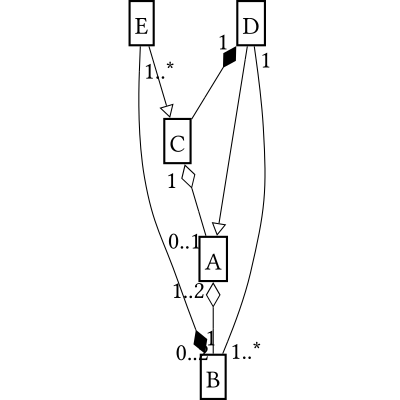
\includegraphics[min width=0.5\textwidth,min height=0.4\textwidth,max width=\textwidth,max height=\textwidth]{53/cd304ec9869e94e1ddda9b2aaa917e2b09bc6fc5eb2c530d1213978d80161cb60e00af83b04c596701db35357ce8aed00a3a92e08161.pdf}}}\figureSeriesRow{\figureSeriesElement{2}{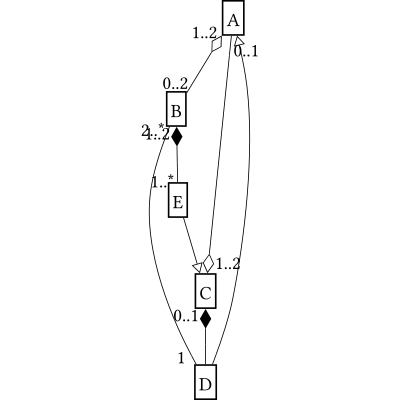
\includegraphics[min width=0.5\textwidth,min height=0.4\textwidth,max width=\textwidth,max height=\textwidth]{53/cd333945a620cbd189ee7844274d4bd715d861613af4941b059ce4cbb4c146d00700af83b04c596701db35357ce8aed00a3a92e08161.pdf}}}\figureSeriesRow{\figureSeriesElement{3}{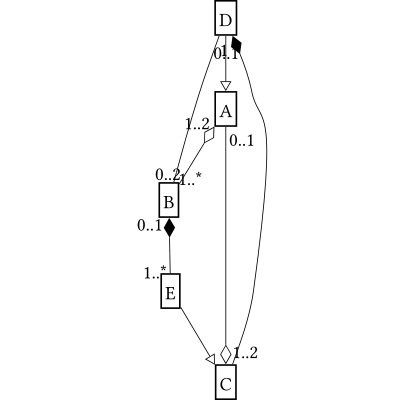
\includegraphics[min width=0.5\textwidth,min height=0.4\textwidth,max width=\textwidth,max height=\textwidth]{53/cd2e8a7356da1b2190494f108e74f5b559583e061c12d76ad31f31c496110002d300af83b04c596701db35357ce8aed00a3a92e08161.pdf}}}\figureSeriesRow{\figureSeriesElement{4}{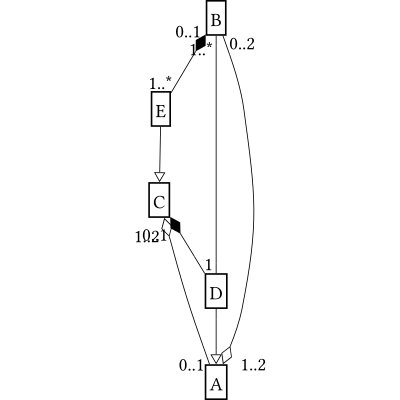
\includegraphics[min width=0.5\textwidth,min height=0.4\textwidth,max width=\textwidth,max height=\textwidth]{53/cdf8026e55054824c5b00dbd86a11a47c0e778bb39e7041008f6001317a9eed28f00af83b04c596701db35357ce8aed00a3a92e08161.pdf}}}}Which of these class diagram candidates are valid class diagrams?
Please state your answer by giving a list of numbers, indicating all valid class diagrams.

For example,\begin{verbatim}[1, 2]\end{verbatim}would indicate that only class diagram candidates 1 and 2 of the given ones are valid class diagrams.

Please note: Classes are represented simplified here. 
 That means they consist of a single box containing only the class name but no sections for attributes or methods. 
 Nevertheless you should treat these simplified class representations as valid classes.

Please note: When hovering over or clicking on edges / nodes or their labels, the respective components that belong together are highlighted.

